\documentclass[12pt]{article}


\title{Unixcrypt Multi-block Analysis}
\date{Dalhousie University} % Aug 2019
\author{Charlie Gerrie}
\usepackage[utf8]{inputenc}


\usepackage{amsthm}
\usepackage{amsmath}
\usepackage{yfonts}
\usepackage{amssymb}
\usepackage{fullpage}
\usepackage{mathtools}
\usepackage{tikz}
\usepackage{graphicx}
\usepackage{subcaption}
\usepackage{float}
\usepackage{pgf}
\usepackage{url}
\usetikzlibrary{arrows}
\DeclarePairedDelimiter\ceil{\lceil}{\rceil}
\DeclarePairedDelimiter\floor{\lfloor}{\rfloor}
\pagestyle{empty}

\newcommand{\mset}[1]{\{\!\!\{#1\}\!\!\}}
\newcommand{\sigmahat}{\hat{\sigma}}
\newcommand{\conseq}{\texttt{conseq}}
\newcommand{\inv}{^{-1}}
\newcommand{\s}[1]{\{#1\}}
\newcommand{\bytes}{\mathbb{Z}_{256}}
\newcommand{\coinc}[2]{\texttt{coinc}(#1;#2)}

\newtheorem{theorem}{Theorem}%[section]

\newtheorem{lemma}{Lemma}%[section]

\newtheorem{proposition}{Proposition}%[section]

\newtheorem{corollary}{Corollary}%[section]

\theoremstyle{definition}
\newtheorem{definition}{Definition}%[section]
 
\theoremstyle{remark}
\newtheorem{remark}{Remark}%[section]

\theoremstyle{remark}
\newtheorem{example}{Example}%[section]

\pagenumbering{gobble}
% TODO SHOULD I HAVE PAGE NUMBERS?

\begin{document}

%TITLE PAGE%
\maketitle
\newpage

% TODO ABSTRACT PAGE
\begin{center}{\textbf{Abstract}}\end{center}
This research introduces a method for multi-block analysis of the unix crypt cipher. We extend a single-block algorithm previously developed for this cipher. Taking advantage of how block keys are related to each other, we collect information about the key used to generate them. We then use statistical methods to pick the most likely key. Thus with sufficiently many blocks we can recover the original key and decrypt the ciphertext completely.

\newpage

\section{Preliminaries}

\begin{itemize}

\item
We consider the permutations of $\bytes$ to be all functions $\bytes \to \bytes$. We make use of their group structure under composition, as well as their group action on $\bytes$ by application. We use multiplicative notation for group operations, and exponentiation will represent repeated multiplication (e.g. $\sigma^3=\sigma \sigma \sigma$).
% permutations
\item
We call a pair of elements $(a,b)$ in $\bytes$ a \emph{wire}, with $a$ being the \emph{start-point} and $b$ being the \emph{end-point}. A wire $(a,b)$ is said to be \emph{in} a permutation $\sigma$ if $\sigma(a)=b$. Thus a wire represents a single image-preimage pair of a permutation.
% wires

\item
We associate the elements of $\bytes$ with bytes when considering the implementation of the cipher and breaking algorithm. We also associate them with single characters, which in practice is done using ascii or a similar character encoding.
% bytes correspondence

\item
Multisets will be used in a manner which intuitively expresses a set which can have multiple copies of the same element. Formally, a multiset $X$ of cardinality $|X|$ is the equivalence class of $|X|$-tuples up to permutations. Thus sorting the elements yields a unique representation. We can assign the elements of this sorted tuple indices and treat them like elements of a sequence. An example of this could be letting $x_i$ be the $i$th element of the sorted tuple. We say an element is \emph{in} a multiset if it appears at least once in the tuple. The \emph{multiplicity} of an element is the number of times it appears in the list. 
% multisets

\item
Sequences will be indexed starting at 0. 
% sequences

\item
We will make use of a commutative diagram [1]. Such a diagram is composed of arrows, representing permutations, meeting at vertices. A path of several arrows represents the composition of the permutations of its constituent arrows. Any two paths with the same start-point and end-point are equivalent.

% TODO commutative diagram?

\end{itemize}
\section{The Cipher}
\par
The unixcrypt cipher key is defined by two permutations of $\bytes$ denoted by the characters $\tau$ and $\sigma$. $\tau$ must be a 256-cycle. $\sigma$ must be self-inverse ($\sigma^2=\texttt{id}$) and have no fixed points ($\sigma(x)\neq x$), or in other words it must be entirely composed of 2-cycles.
% TODO put in equations


\par
When using the cipher we will consider two bodies of text, the plaintext and the ciphertext. Both represent sequences of elements in $\bytes$. The ciphertext will be produced from the plaintext by the cipher defined in equation (\ref{ciphereq}). We partition these sequences into segments of 256 elements known as \emph{blocks}. Thus consider $p_i$, the $i$th character of the plaintext. Let $i=256 j + k$, where $0\leq k < 256$. Then $p_i$ is part of the $j$th block of the plaintext, and is the $k$th character within that block.
% define plaintext and ciphertext?
% QUESTION is this necessary?

\par We can then encode $p_i$ into the $i$th character of the ciphertext using this equation:
\begin{equation}
	\label{ciphereq}
	c_i = \kappa^{-k} \tau^{-j} \sigma \tau^j \kappa^k p_i
\end{equation}
where $\kappa$ is the successor function $\kappa(x)=x+1\mod 256 $.


\par
Note that this cipher is symmetric-key, meaning it uses the same key for encryption and decryption. Also, the encryption and decryption processes are the exact same. This follows from equation (\ref{ciphereq}) and the fact that $\sigma^2=\texttt{id}$.
% TODO proof
% TODO refer to sigma squared = 1 equation

\par
Notice that the exponent on $\tau$ is only incremented when $j$ is incremented. This happens every 256 characters. Thus we define the $j$th \emph{block key} $\sigma_j$ by:
\begin{equation}
		\label{blockeq}
		\sigma_j = \tau^{-j} \sigma \tau^j
\end{equation}
This combines both the $\sigma$ and $\tau$ parts of the key into one, giving us a single permutation for encoding the $j$th block. This will be important for using the information from the single-block analysis. Note that $\sigma_0 = \sigma$.
% sigma_j and sigma_j hat

\section{Single-Block Analysis}
\par
Previous work on this cipher has produced a method of single-block analysis [2]. This looks at each block individually and tries to find, or in practice approximates, the block keys for each block. Thus, we obtain approximations of each block key $\sigma_j$, which we will denote $\hat{\sigma}_j$. 
% single-block analysis
% TODO outline more!

\par
Each block only consists of 256 characters, so on average every wire is used just once.
% TODO finish
% QUESTION rational for 
In practice what this means is that the single-block analysis can successfully reproduce about half of the wires in each block key. It also makes a small number of incorrect guesses, and leaves the rest of the wires unguessed. This last part is insignificant when the single-block analysis is performed by itself, but to perform the multi-block analysis we will need the block key approximations to be complete permutations so we can perform calculations with them. Thus, to "fill out" the permutations we assign the unguessed wires at random. This can be done efficiently with a Fisher-Yates shuffle.
% success

\par
% TODO other methods not involving filling

\section{Multi-block Analysis}
\par
% general description

\par
The input to the algorithm is a collection of block key approximation. We get these by running the single-block analysis on the ciphertext first. 
%input

\par
output
%output

\par
goal
%goal
\section{Coincidences}
\par
% TODO intro

\par
We define an indicator function $\delta$ taking two arguments $x$ and $y$
\[
	\delta(x,y)=
	\begin{cases}
		1 & \texttt{if}\ x=y \\
		0 & \texttt{if}\ x \neq y
	\end{cases}
\]
Then for any two multisets $X$ and $Y$ with elements $x_i$ and $y_j$, where $0\leq i < |X|$ and $0\leq j < |Y|$, we define their \emph{coincidence} as:
\begin{equation}
	\coinc{X}{Y} = \sum_{i,j} \delta(x_i,y_j)
\end{equation}
with the sum being over all possible pairs of $i$ and $j$.

\par
To demonstrate the principle of what we will be doing, let us consider this example. You have two bags of size $k$ and $k^2$ each filled with labelled objects. If you didn't know which bag you had, could you \emph{guess} only by sampling from the bags and counting the number of coincidences in the objects drawn? The answer is yes. If we pulled an object out the the bag, recorded which one it was, returned it, then drew another item, what would be the probability they were the same one? Well if we had the bag with $k$ objects it would be $\frac{1}{k}$, but if we had the bag with $k^2$ objects it would be $\frac{1}{k^2}$. These values will be very different, so by sampling many times we can see whether the probability that we get two matching objects is closer to $\frac{1}{k}$ or $\frac{1}{k^2}$ and thus determine which bag we probably have.
% coincedences example?
% Does this belong here or somewhere else, esp because of reference to statistical testing?

\subsection{Coincidences and the Algorithm}
\par
Figure \ref{ladderfig} shows a commutative diagram derived from equation (\ref{blockeq}). Of particular note is the equivalence of $\tau$ and $\sigma_1 \tau \sigma^{-1}_0$, marked in red and blue respectively. Thus, if we conjecture that $(a,b)$ is a wire in $\tau$ then it must also be a wire in $\sigma_1 \tau \sigma^{-1}_0$. But the wire in $\sigma_1 \tau \sigma^{-1}_0$ is really three wires: a wire $(a,\sigma_1(a))$ in $\sigma_1$, a wire $(\sigma_1(a),\sigma_0(b))$ in $\tau$, and a wire $(\sigma_0(b), b)$ in $\sigma^{-1}_0$. Thus, if $(a,b)$ is a wire in $\tau$ then $(\sigma_1(a),\sigma_0(b))$ must also be a wire in $\tau$. In general, all wires $(\sigma_{i+1}(a),\sigma_i(b))$ must be in $\tau$. Thus, the \emph{wire consequences} of $(a,b)$ are all the wires that must also be in $\tau$ if $(a,b)$ is.

% explain ladder diagram
\begin{figure}[h!]
	\centering
	\caption{}
	\label{ladderfig}
	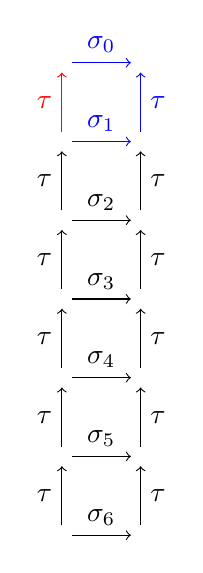
\begin{tikzpicture}[node distance=10pt]
		\foreach \i in {0,...,6} {
			\node (L\i) at (0,-\i) {};
			\node (R\i) at (1,-\i) {};
		}
		\foreach \i in {0,...,5} {
			\node (BL\i) at (0,-\i-1) {};
			\node (BR\i) at (1,-\i-1) {};
		}
		\draw [red, arrows={->}] (BL0) edge node[left] {$\tau$} (L0);
		\draw [blue, arrows={->}] (L0) edge node[above] {$\sigma_0$} (R0);
		\draw [blue, arrows={->}] (BR0) edge node[right] {$\tau$} (R0);
		\draw [blue, arrows={->}] (L1) edge node[above] {$\sigma_1$} (R1);
		\foreach \i in {2,...,6} {
			\draw [->] (L\i) edge node[above] {$\sigma_\i$} (R\i);
		}
		\foreach \i in {1,...,5} {
			\draw [->] (BL\i) edge node[left] {$\tau$} (L\i);
			\draw [->] (BR\i) edge node[right] {$\tau$} (R\i);
		}
	\end{tikzpicture}
\end{figure}
\begin{definition}[Wire Consequences]
	For a wire $(a,b)$, we have
	\begin{equation}
		\conseq(a,b)=\mset{\sigmahat_i(a), \sigmahat_{i+1}(b)) : 0\leq i<N-1}\end{equation}
	where $N$ is the number of $\sigmahat$'s. This is a multiset.
\end{definition}





\par
TODO Explain why coincidences






\begin{definition}[Wire-to-wire Coincidences]
	If we consider two wires $(a,b)$ and $(c,d)$, then we have
	\begin{equation}
		\label{coinceq}
		\texttt{coinc}(a,b,c,d)=\sum^{255}_{i=0} \sum^{255}_{j=0} \texttt{conseq}(a,b)_{i,j} \texttt{conseq}(c,d)_{i,j}
	\end{equation}
	where $\texttt{conseq}(a,b)_{i,j}$ is the multiplicity of the wire $(i,j)$ in the consequences of $(a,b)$.
% TODO equation
	This is a count of all the possible pairs of similar elements in the two wires consequence multisets. 
\end{definition}
\begin{figure}[h!]
	\centering
	\caption{}
	\label{coincfig}
	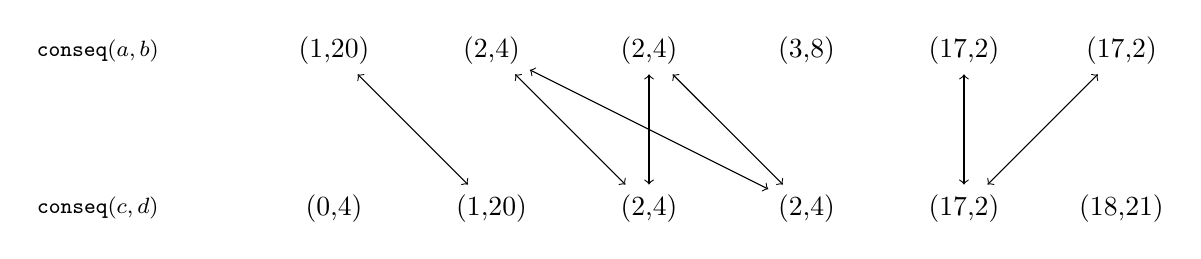
\begin{tikzpicture}
		\node (cons1) at (-3,0) {\begin{footnotesize}$\texttt{conseq}(c,d)$\end{footnotesize}};
		\node (cons2) at (-3,2) {\begin{footnotesize}$\texttt{conseq}(a,b)$\end{footnotesize}};	
	
		\node (T1) at (0,0) {(0,4)};
		\node (T2) at (2,0) {(1,20)};
		\node (T3) at (4,0) {(2,4)};
		\node (T4) at (6,0) {(2,4)};
		\node (T5) at (8,0) {(17,2)};
		\node (T6) at (10,0) {(18,21)};
		\node (B1) at (0,2) {(1,20)};
		\node (B2) at (2,2) {(2,4)};
		\node (B3) at (4,2) {(2,4)};
		\node (B4) at (6,2) {(3,8)};
		\node (B5) at (8,2) {(17,2)};
		\node (B6) at (10,2) {(17,2)};
		
		\draw [<->] (T2) -- (B1);
		\draw [<->] (T3) -- (B2);
		\draw [<->] (T4) -- (B2);
		\draw [<->] (T3) -- (B3);
		\draw [<->] (T4) -- (B3);
		\draw [<->] (T5) -- (B5);
		\draw [<->] (T5) -- (B6);
	\end{tikzpicture}
\end{figure}
% TODO FIGURE arrows for pairing up

\par
Figure \ref{coincfig} shows how we count the possible pairs. This example would be expressed as an expansion of equation (\ref{coinceq}) as follows:
\begin{equation}
\begin{split}
	\texttt{coinc}(a,b,c,d) =& \sum^{255}_{i=0} \sum^{255}_{j=0} \texttt{conseq}(a,b)_{i,j} \texttt{conseq}(c,d)_{i,j} \\ =& \texttt{conseq}(a,b)_{1,20} \texttt{conseq}(c,d)_{1,20} + \texttt{conseq}(a,b)_{2,4} \texttt{conseq}(c,d)_{2,4} \\ & + \texttt{conseq}(a,b)_{17,2} \texttt{conseq}(c,d)_{17,2} \\  = & (1)(1) + (2)(2) + (2)(1) \\  = & 7
\end{split}
\end{equation}
with all other terms in the sums evaluating to zero.

\par
Finally, it should be noted that wire-to-wire coincidences are always non-negative integers.


\begin{definition}[Coincidences Distribution]
	Given a wire, we can define a discrete distribution of the value of the wire-to-wire coincidences between that wire and another randomly chosen wire.
\end{definition}
% TODO equation?
% TODO FIGURE example histogram? 
\par
Here is an example the coincidences distribution for a wire (75,29), encoding the probability of each number of wire-to-wire coincidences between (75,29) and a randomly chosen wire (c,d).
\begin{center}
\begin{tabular}{|c|c|c|c|c|}
\hline
$X$ & 0 & 1 & 2 & ... \\
\hline 
$P(\texttt{coinc}(75,29,c,d)=X)$ & 0.933 & 0.0648 & 0.00224 & ... \\

\hline
\end{tabular}
\end{center}
% TODO facts and general shape
Notice that it is very likely that the number of wire-to-wire coincidences is 0, and that the probability falls of sharply as the number of coincidences increases. Note that in practice we generate this distribution by sampling the wire-to-wire coincidences between the given wire $(a,b)$ and wires $(c,d)$ that satisfy the following conditions: $a\neq b$ and $c\neq d$ because $\tau$ is a 256-cycle and cannot have fixed points, and $a\neq c$ and $b \neq d$ because then they would be mutually exclusive. There are 64771 such wires. 

\par
Now to reconstruct $\tau$, we need to find all 256 of its wires. To do this, we calculate the coincidences distribution for all possible wires, of which there are $256 \times 255$ since wires in $\tau$ cannot connect to themselves. Then for all 256 wire start-points, we will pick the best end-point using the coincidences distribution. This will give us our guess at $\tau$.
% describe algorithm
% process by which we run these things for all values of a hypothetical tau


\section{Likelihood}
\subsection{Likelihood and the Algorithm}




\par
To rigorously determine which distribution our sample distribution fits, we will be using a concept from statistics and probability theory known as \emph{likelihood}. If we consider two events $A$ and $B$, then likelihood is related to conditional probability by the relation 
\[ \mathcal{L}(A|B)=P(B|A)\]
Now we have two potential distributions and we would like to know which one our sample distribution follows. Let $D_1$ and $D_2$ be the events that the sample distribution follows the two distributions and $S$ is the event of getting the samples that we did. We would like to calculate $P( D_1 |S)$ and $P( D_2 | S)$ and then choose the distribution with the higher probability. Now it is easy to calculate $P(S | D_1 )$ and $P(S | D_2 )$. Assuming the samples are independent, they are simply the products of the pdf values for all the samples. Normally we would then use Bayes' theorem:
\[ P(D_1 | S) = \frac{P(S | D_1) P(D_1)}{P(S)} \]
But this would require us to know an \emph{a priori} probability of the distribution and the samples. This we cannot know, so Bayes' theorem fails us. 

\par
This is where likelihood comes to the rescue. The probabilities we can calculate, $P( S | D_1)$ and $P( S | D_2 )$, are precisely the likelihoods $\mathcal{L}(D_1 | S)$ and $\mathcal{L}(D_2 | S)$. Since we cannot choose the most \emph{probable} distribution of the two, we choose the most \emph{likely}. This is known as the maximum likelihood method [3].
% TODO REFERENCE
% explain likelihood
% maximum likelihood method/principle


\par
Now our problem is that for each wire start-point we have 255 possible end-points. Each end-point defines a potential wire with a coincidences distribution. For each wire we consider the question "is this wire actually in $\tau$ or not?" Let the null hypothesis be that it is an incorrect guess and is not in $\tau$, and the alternative hypothesis be that it is in $\tau$. The next step would be to construct hypothetical distributions for both cases, but constructing the distribution for the alternative hypothesis is complicated and there is a simpler way. We can easily construct a distribution for the null hypothesis, which we will call the \emph{null distribution}, and we can choose the wire which is least likely to fit this distribution and fulfill the null hypothesis.

\par
If a wire is not in $\tau$, then the logic behind its wire consequences also being in $\tau$ does not apply. Its consequences are then essentially random, so they are chosen from all $256\times 256$ pairs

TODO FINISH


Thus the null distribution depends on the number of blocks being analyzed since that determines the number of wire consequences each wire has.
% null distribution
% TODO FIGURE
\begin{center}
\begin{tabular}{|c|c|c|c|c|}
\hline
$X$ & 0 & 1 & 2 & ... \\
\hline 
$P(\texttt{coinc}(a,b,c,d)=X)$ & 0.965 & 0.0345 & 0.000618 & ... \\

\hline
\end{tabular}
\end{center}

\par
% correct wire
% it's actually 64771 samples
% TODO FIGURE

\par
TODO number of blocks required
% number of blocks
% FIGURE graph

\section{Finding $\sigma$}

\par
We can restate equation (\ref{blockeq}) as follows
\[ \sigma = \tau^j \sigma_j \tau^{-j} \]
Then once we have determined $\tau$ we can recombine it with the block key approximations from the single-block analysis to get a collection of approximations for $\sigma$. Then for each wire start-point we pick the end-point that occurs the most times in these approximations.

% 

% TODO how few can this be done with?

\section{Conclusion}

\section{Appendix: Tail Density?}
\section{Appendix: Code?}
% TODO APPENDIX FOR TAIL DENSITY IMPROVEMENT?
APPENDIX FOR K sigmastotau DATA STRUCTURE IMPROVEMENT?
\section{References}

[1] http://mathworld.wolfram.com/CommutativeDiagram.html \\ 

\noindent
[2] https://www.mathstat.dal.ca/$\sim$selinger/unixcrypt-breaker/ \\

\noindent
[3] http://mathworld.wolfram.com/MaximumLikelihood.html
\end{document}
